\documentclass[12pt,a4paper]{article}

% \usepackage[utf8]{inputenc}
% \DeclareUnicodeCharacter{1D12A}{\doublesharp}
% \DeclareUnicodeCharacter{2693}{\anchor}
% \usepackage{dingbat}
% \DeclareRobustCommand\dash\unskip\nobreak\thinspace{\textemdash\allowbreak\thinspace\ignorespaces}
% \usepackage[top=1in, bottom=1in, left=1in, right=1in, headheight=15pt]{geometry}
%\usepackage{fullpage}

\usepackage{tabularx}
\usepackage{multirow}
\usepackage{makecell}
\usepackage{fancyhdr}\pagestyle{fancy}\rhead{Stephanie Wang}\lhead{AWM Travel Grant -- Research Proposal}

\usepackage{amsmath,amssymb,amsthm,amsfonts,microtype,stmaryrd,mathtools}
	%{wasysym,yhmath}

\usepackage[usenames,dvipsnames]{xcolor}
\newcommand{\blue}[1]{\textcolor{blue}{#1}}
\newcommand{\red}[1]{\textcolor{red}{#1}}
\newcommand{\gray}[1]{\textcolor{gray}{#1}}
\newcommand{\fgreen}[1]{\textcolor{ForestGreen}{#1}}

\usepackage{mdframed}
	%\newtheorem{mdexample}{Example}
	\definecolor{warmgreen}{rgb}{0.8,0.9,0.85}
	% --Example:
	% \begin{center}
	% \begin{minipage}{0.7\textwidth}
	% \begin{mdframed}[backgroundcolor=warmgreen, 
	% skipabove=4pt,skipbelow=4pt,hidealllines=true, 
	% topline=false,leftline=false,middlelinewidth=10pt, 
	% roundcorner=10pt] 
	%%%% --CONTENTS-- %%%%
	% \end{mdframed}\end{minipage}\end{center}	

\usepackage{graphicx} \graphicspath{{}}
	% --Example:
	% \includegraphics[scale=0.5]{picture name}
%\usepackage{caption} %%% --some awful package to make caption...

\definecolor{darkblue}{rgb}{0.2,0.2,0.5}
\usepackage[unicode]{hyperref}\hypersetup{linktocpage,colorlinks}\hypersetup{citecolor=black,filecolor=black,linkcolor=black,urlcolor=blue,breaklinks=true}

%%% --Text Fonts
%\usepackage{times} %%% --Times New Roman for LaTeX
%\usepackage{fontspec}\setmainfont{Times New Roman} %%% --Times New Roman; XeLaTeX only

%%% --Math Fonts
\renewcommand{\v}[1]{\ifmmode\mathbf{#1}\fi}
\renewcommand{\b}[1]{\ifmmode\boldsymbol{#1}\fi}
%\renewcommand{\mbf}[1]{\mathbf{#1}} %%% --vector
%\newcommand{\ca}[1]{\mathcal{#1}} %%% --"bigO"
%\newcommand{\bb}[1]{\mathbb{#1}} %%% --"Natural, Real numbers"
%\newcommand{\rom}[1]{\romannumeral{#1}} %%% --Roman numbers

%%% --Quick Arrows
\newcommand{\ra}[1]{\ifnum #1=1\rightarrow\fi\ifnum #1=2\Rightarrow\fi\ifnum #1=3\Rrightarrow\fi\ifnum #1=4\rightrightarrows\fi\ifnum #1=5\rightleftarrows\fi\ifnum #1=6\mapsto\fi\ifnum #1=7\iffalse\fi\fi\ifnum #1=8\twoheadrightarrow\fi\ifnum #1=9\rightharpoonup\fi\ifnum #1=0\rightharpoondown\fi}

%\newcommand{\la}[1]{\ifnum #1=1\leftarrow\fi\ifnum #1=2\Leftarrow\fi\ifnum #1=3\Lleftarrow\fi\ifnum #1=4\leftleftarrows\fi\ifnum #1=5\rightleftarrows\fi\ifnum #1=6\mapsfrom\ifnum #1=7\iffalse\fi\fi\ifnum #1=8\twoheadleftarrow\fi\ifnum #1=9\leftharpoonup\fi\ifnum #1=0\leftharpoondown\fi}

%\newcommand{\ua}[1]{\ifnum #1=1\uparrow\fi\ifnum #1=2\Uparrow\fi}
%\newcommand{\da}[1]{\ifnum #1=1\downarrow\fi\ifnum #1=2\Downarrow\fi}

%%% --Special Editor Config
\renewcommand{\ni}{\noindent}
\newcommand{\onum}[1]{\raisebox{.5pt}{\textcircled{\raisebox{-1pt} {#1}}}}

\newcommand{\claim}[1]{\underline{``{#1}":}}

\renewcommand{\l}{\left}\renewcommand{\r}{\right}\newcommand{\m}{\middle}

\newcommand{\casebrak}[4]{\left \{ \begin{array}{ll} {#1},&{#2}\\{#3},&{#4} \end{array} \right.}
%\newcommand{\ttm}[4]{\l[\begin{array}{cc}{#1}&{#2}\\{#3}&{#4}\end{array}\r]} %two-by-two-matrix
%\newcommand{\tv}[2]{\l[\begin{array}{c}{#1}\\{#2}\end{array}\r]}

\def\dps{\displaystyle}

\let\italiccorrection=\/
\def\/{\ifmmode\expandafter\frac\else\italiccorrection\fi}


%%% --General Math Symbols
\def\bc{\because}
\def\tf{\therefore}

%%% --Frequently used OPERATORS shorthand
\newcommand{\INT}[2]{\int_{#1}^{#2}}
\newcommand{\Int}[1]{\int_{#1}}
% \newcommand{\UPINT}{\bar\int}
% \newcommand{\UPINTRd}{\overline{\int_{\bb R ^d}}}
\newcommand{\SUM}[2]{\sum\limits_{#1}^{#2}}
\newcommand{\PROD}[2]{\prod\limits_{#1}^{#2}}
\newcommand{\CUP}[2]{\bigcup\limits_{#1}^{#2}}
\newcommand{\CAP}[2]{\bigcap\limits_{#1}^{#2}}
% \newcommand{\SUP}[1]{\sup\limits_{#1}}
% \newcommand{\INF}[1]{\inf\limits_{#1}}
\newcommand{\pd}[2]{\frac{\partial{#1}}{\partial{#2}}}
\def\tr{\text{tr}}

\renewcommand{\o}{\circ}
\newcommand{\x}{\times}
\newcommand{\ox}{\otimes}

\newcommand\ie{{\it i.e. }}
\newcommand\wrt{{w.r.t. }}
\newcommand\dom{\mathbf{dom\:}}

%%% --Frequently used VARIABLES shorthand
\newcommand{\R}{\ifmmode\mathbb R\fi}
\newcommand{\N}{\ifmmode\mathbb N\fi}
\newcommand{\T}{\ifmmode\mathbb T\fi}
\renewcommand{\O}{\mathcal{O}}
\newcommand{\w}{\wedge}
\newcommand{\ome}{\omega}
\newcommand{\lam}{\lambda}
\newcommand{\im}{\mbox{im}}

\newcommand{\B}{\mathcal B}

%============================
% Conjugate, Double bracket
%============================

\makeatletter
\DeclareFontFamily{OMX}{MnSymbolE}{}
\DeclareSymbolFont{MnLargeSymbols}{OMX}{MnSymbolE}{m}{n}
\SetSymbolFont{MnLargeSymbols}{bold}{OMX}{MnSymbolE}{b}{n}
\DeclareFontShape{OMX}{MnSymbolE}{m}{n}{
    <-6>  MnSymbolE5
   <6-7>  MnSymbolE6
   <7-8>  MnSymbolE7
   <8-9>  MnSymbolE8
   <9-10> MnSymbolE9
  <10-12> MnSymbolE10
  <12->   MnSymbolE12
}{}
\DeclareFontShape{OMX}{MnSymbolE}{b}{n}{
    <-6>  MnSymbolE-Bold5
   <6-7>  MnSymbolE-Bold6
   <7-8>  MnSymbolE-Bold7
   <8-9>  MnSymbolE-Bold8
   <9-10> MnSymbolE-Bold9
  <10-12> MnSymbolE-Bold10
  <12->   MnSymbolE-Bold12
}{}
\let\llangle\@undefined
\let\rrangle\@undefined
\DeclareMathDelimiter{\llangle}{\mathopen}%
                     {MnLargeSymbols}{'164}{MnLargeSymbols}{'164}
\DeclareMathDelimiter{\rrangle}{\mathclose}%
                     {MnLargeSymbols}{'171}{MnLargeSymbols}{'171}
\makeatother

\title{AWM Travel Grant -- Research Proposal}
\author{Stephanie Wang}
\date{\today}

% The following lines include both bibentry and hyperref packages while resolving the clash
% See https://tex.stackexchange.com/questions/65348/clash-between-bibentry-and-hyperref-with-bibstyle-elsart-harv
\usepackage{bibentry} % using BibTeX for publication list
\makeatletter\let\saved@bibitem\@bibitem\makeatother

\begin{document}
This is a research proposal where I present the rationale of funding my travel to Tokyo in August of 2023 to attend the 10th International Congress on Industrial and Applied Mathematics (ICIAM). 
During my attendance, I will present a talk titled ``Capturing surfaces using differential forms''.  
The talk will be a part of the \emph{Computational methods for interfaces in physics and mechanics} minisymposium, which is organized by \href{http://www.cmap.polytechnique.fr/~antonin/}{Prof. Antonin Chambolle} and \href{https://ms.mcmaster.ca/~bourdinb/}{Prof. Blaise Bourdin}.  
 
The talk that I am preparing to present is based on my recent paper, \href{https://dl.acm.org/doi/10.1145/3450626.3459781}{Computing minimal surfaces with differential forms}, originally published in \emph{ACM Transactions on Graphics} \cite{Wang:2021}.
In the paper, my co-author and I explored a new numerical representation of geometries (curves and surfaces) called \emph{current}, which originated from the study of geometric measure theory (GMT).  
In physics and mechanics, researchers are often studying the evolution of a surface or an optimization problem where the geometry itself is the variable.   
Existing numerical representations of geometries (surfaces and curves) either explicitly store positions of the vertices and a combinatorial structure of the connectivity, or implicitly encode the geometries as the level set of a function, lacking the capacity to represent geometries with nonempty boundaries.  
Our GMT-based representation simultaneously provides the capacity of representing geometries with boundaries as well as the convenience of continuous and differentiable changes in topology.  
We demonstrate in our paper how this new geometry representation applies to the classical Plateau problem, the problem of finding the surface of minimal area subject to a prescribed boundary curve (or a prescribed set of boundary curves). 
Our geometry representation allows us to continuously search for solutions of a variety of topologies, bypassing all re-meshing steps in existing algorithms like \cite{pinkall1993minsurfaces}.   
Furthermore, the GMT-based representation mirrors the view point of simplicial geometry where the boundary operator is linear.  
As a result, we convert the classically nonconvex Plateau problem into a textbook convex problem-- a convex, norm-like functional to minimize, along with a linear constraint.  
Our computational method utilizes the recent development of Alternating Direction Method of Multipliers (ADMM) \cite{Goldstein:2014:ADMM} and Fast Fourier Transform (FFT), making the minimization process both fast and robust.  
In addition, I will also cover an extended work in my talk, \href{https://openaccess.thecvf.com/content/CVPR2022/papers/Palmer_DeepCurrents_Learning_Implicit_Representations_of_Shapes_With_Boundaries_CVPR_2022_paper.pdf}{DeepCurrents: Learning Implicit Representations of Shapes with Boundaries}.  
In the extended work, my co-authors and I used Fourier features together with deep neural network to discretize currents to achieve infinite resolution as well as a data-driven auto-encoder of surfaces with boundaries \cite{Palmer:2022}. 

The GMT-based geometry representation has a lot of potential for future computational methods, for its flexibility with topology changes, differentiability, and an easy linear operator to compute the boundaries.  
In Computer Vision, researchers are always searching for better numerical representations for geometries \cite{mildenhall2020nerf, takikawa2021nglod, meng2023neat}, aiming to solve problems in inverse-rendering, relighting, and generative models for geometries.  
My talk at ICIAM is a valuable opportunity to for me to reach and exchange ideas with mathematicians outside the community of computer graphics and computer vision, which is where my original papers were published. 
In particular, computations involving geometries is a fundamental problem in almost all numerical methods in physics and mechanics. 
This is especially true in the modeling of material fracture, with which I had direct research experience and proposed a complicated method to track the topological changes of an evolving fracture interface \cite{Wang:2019}. 


Attached below are rendered images of our computational results of Plateau problems. 
I appreciate AWM's consideration of my application, and I look forward to hearing from the award committee. 
\begin{figure*}[h]
  \centering
    \includegraphics[width=0.4\linewidth]{Borromean_DGD_calendar_powerplant_blue.png}
    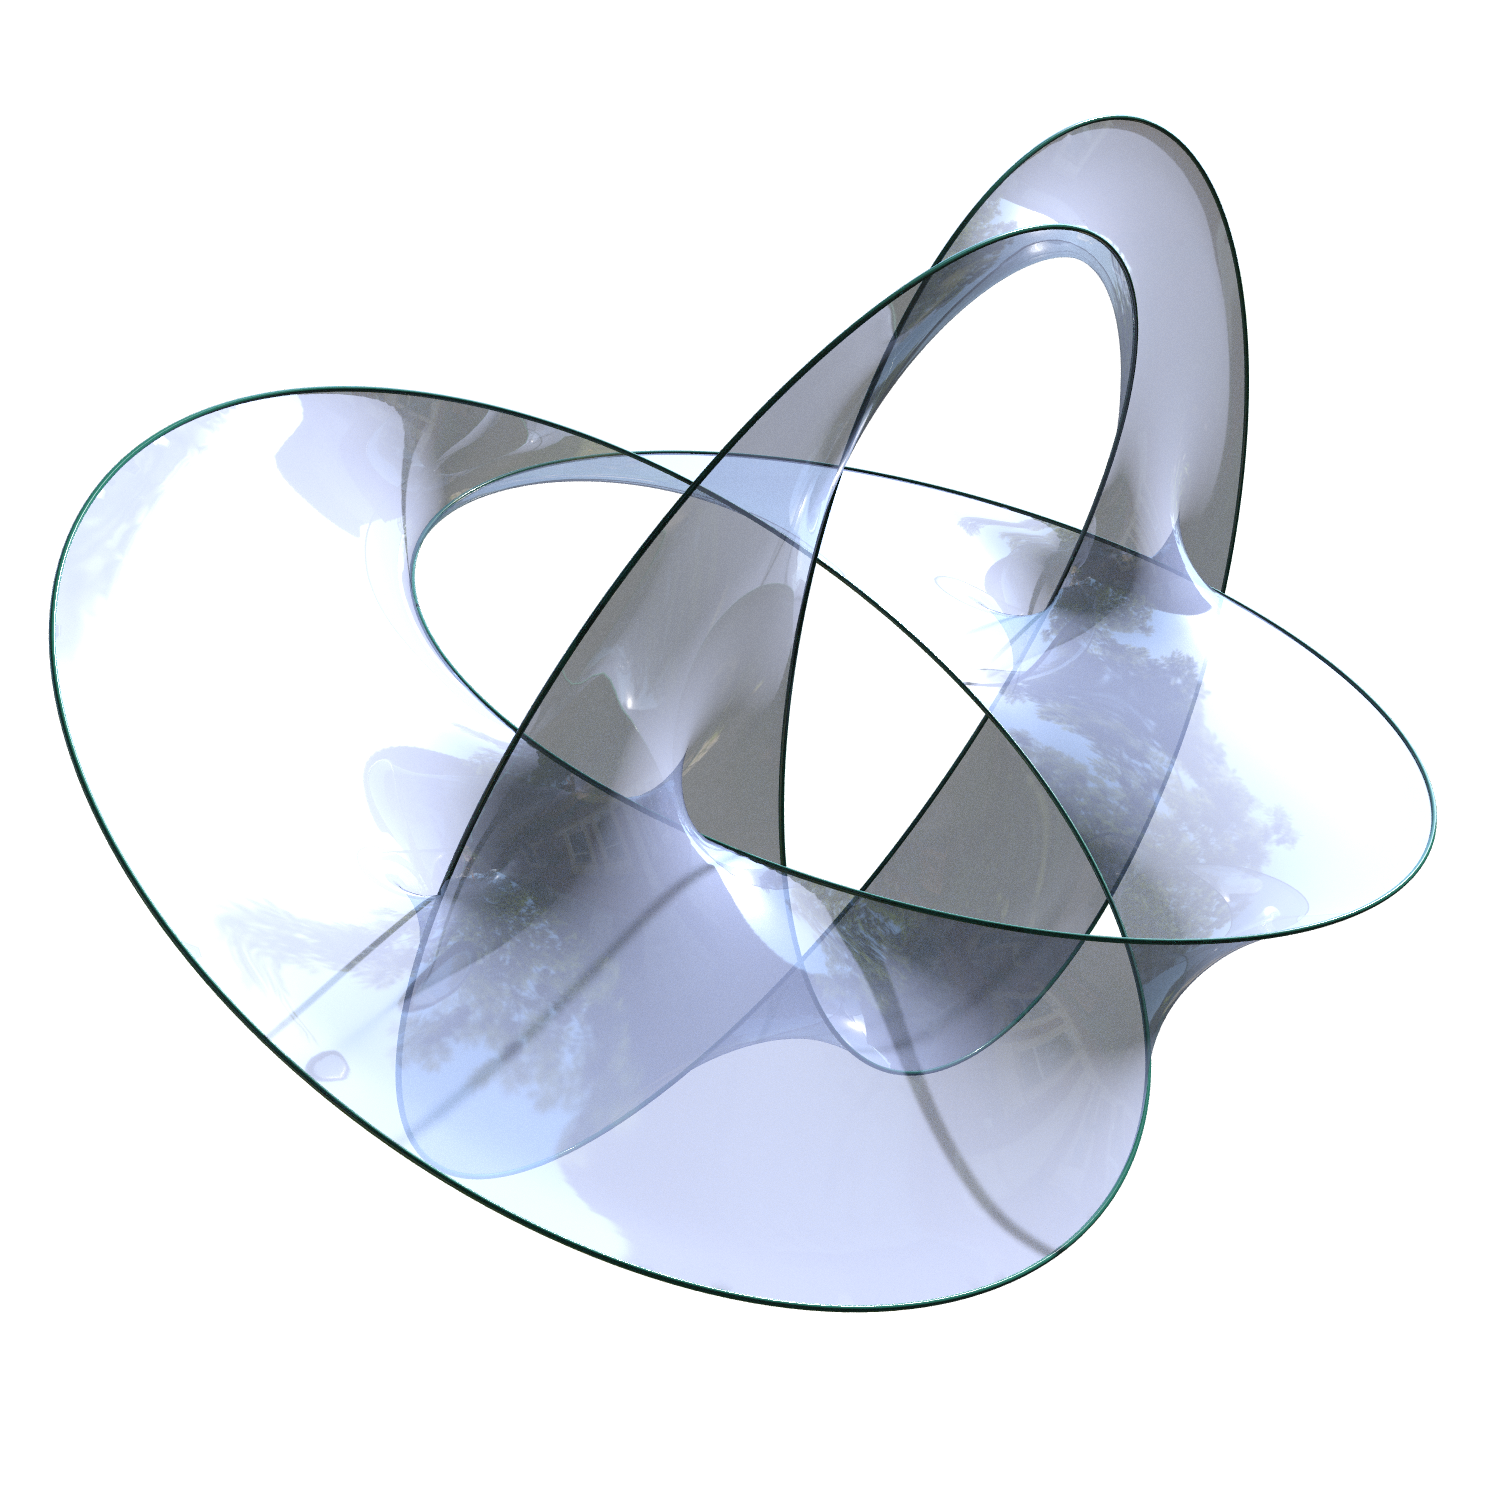
\includegraphics[width=0.4\linewidth]{DGD_calendar_collage_rings_surface.png}
    \caption{
      Predicting the topology of the solution to Plateau problem has always been a difficult problem. Our computational method can handle arbitrary boundary curves and always find the global minimizer for Plateau problem. Left: minimal surface with boundary prescribed as the Borromean rings (prescribed in squared shapes). Right: minimal surface with boundary prescribed as five arbitrarily positioned circles. 
    }
  \end{figure*}

\bibliographystyle{plain}
\bibliography{PublicationsAndCitations}
\end{document}
